\begin{center}
	
	\begin{tabular}{rp{16cm}lp{20cm}}%{rl}
		
		% after \\: \hline or \cline{col1-col2} \cline{col3-col4} ...
		
		论文地址:& \href{https://web.stanford.edu/~cpiech/bio/papers/deepKnowledgeTracing.pdf}{https://web.stanford.edu/~cpiech/bio/papers/deepKnowledgeTracing.pdf} \\
		来源:& NIPS, 2015 \\
		作者:& Chris Piech, et al. \\
		单位:& Stanford University, Khan Academy, Google \\
		源码:& \href{https://github.com/chrispiech/DeepKnowledgeTracing}{DeepKnowledgeTracing-lua}、\href{https://github.com/siyuanzhao/2016-EDM}{DeepKnowledgeTracing-py}\\
		
		%  slides:& \href{http://yunshengb.com/wp-content/uploads/2017/03/nips_2018_r2l_workshop_talk.pdf}{{\footnotesize Convolutional Set Matching for Graph Similarity}}\\
		
		关键词:& \textbf{Knowledge Tracing, RNN} \\
		
		写于:& \date{2021-09-22}
		
	\end{tabular}
	
\end{center}

该论文\cite{piech2015deep}使用RNN来对学生的知识水平进行追踪(Knowledge Tracing),提出了Deep Knowledge Tracing(DKT) --- 用RNN来捕捉学生与课程的交互序列,将学生的知识表示为可以学习的embedding。

\paragraph{问题定义}
\textbf{Knowledge Tracing(KT))}旨在对学生的只是进行建模,追踪学生的知识水平是如何随着与学生与课程交互而变化的。

能够准确地追踪学生的知识,有助于发现学生在学习过程中的薄弱点,更准确的引导学生学习 --- 有哪些知识点薄弱、哪些知识点已经掌握,更有针对性的查漏补缺。

KT的难点在于人类学习过程的复杂以及知识的表示的复杂:
\begin{itemize}
	\item 学习的过程是复杂的,涉及到多种对象
	\item 如何表示人的学习过程
	\item 人的知识水平如何体现
	\item 被学习的技能如何划分
	\item 学习材料如何学习内容相对应
	\item 人类在多种资料上学习:听说读写,甚至有动作,如何在在这些载体上追踪学生的知识
\end{itemize}


\textbf{形式化定义}:
在某个学习任务上,学生持续与相关的课程进行交互 --- 通常指做题,预测学生下一时刻回答某问题正确的概率。学生与课程的交互序列:$\boldsymbol{x_0}, \boldsymbol{x_1}, ..., \boldsymbol{x_t}$,通常$\boldsymbol{x_t} = \{q_t, a_t\}$表示$t$时学生做的题目以及学生的答案。

这篇论文的目的是\tbc{red}{基于学生以往的交互,预测学生对练习的作答情况}。

\paragraph{DKT}
DKT的模型比较简单,如Fig.\ref{fig:dkt}所示,有两个版本:一个基于普通的RNN、一个基于LSTM。

\begin{figure}[h]
	\centering
	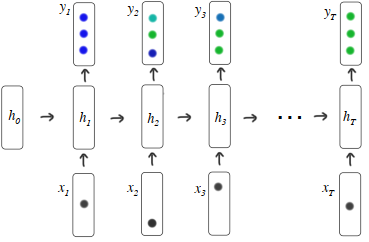
\includegraphics[width=.35\textwidth]{pics/dkt.png}
	\caption{Deep Knowledge Tracing}
	\label{fig:dkt}
\end{figure}

模型的输入是学生的交互序列。DKT设定一共有$M$个练习,学生的每一次交互表示为:$\boldsymbol{x_t} = \{q_t, a_t\} \in \mathbb{R}^{2M}$。$q_t$表示学生回答的问题,$a_t$表示学生的作答,分别用one-hot表示。但是当$M$很大时,往往会带来过多的参数、难以训练等问题,因此,论文用一个dense vector表示一交互:$\boldsymbol{x_t} = \boldsymbol{n}_{q_t, q_t} \sim \mathcal{N}(0, \boldsymbol{I})$。

训练过程中使用交叉熵损失,评测指标是AUC。使用的数据集有:人工生成的模拟数据、Khan Academy Data、\href{https://sites.google.com/site/assistmentsdata/home/assistment-2009-2010-data}{Assistments benchmark dataset}。


\paragraph{总结}

\begin{itemize}
	\item 无需对练习进行标注(标注每个练习对应的知识点)
	\item 可以用于发现练习之间的关系 
	\item 第一个使用深度模型做Knowledge Tracing的
\end{itemize}

